\chapter{Image Analysis}\label{chapter3}

In this chapter, we analyze container images, which are used in
%In comparison, no vulnerabilities were found in base
%Docker images \texttt{ubuntu:20.04} and \texttt{centos:7} after package
%update.two neuroscience containerization frameworks, are analyzed for
two neuroscience frameworks. In accordance with that, these
images are scanned using four popular scanners. Additionally,
two different approaches, \textit{image update} and \textit{
image minification} are followed in order to see their
effect on the security vulnerabilities. Finally, this
chapter discuss results of
these experiments.

\section{Image Scanning}
Image scanning is a technique to
detect image vulnerabilities, which reduces the risk of vulnerability exploitation
inside containers. Scanning refers to the practice of collecting all
information about the container image,
investigating it for
vulnerabilities, and finally producing a report to
summarize scanning results. These reports can be used for security assessments.
%According to Docker Hub's statistics, it has 100K+ repositories consisting
%of 900K+ public images having 12+ billion image pulls every week~\cite{xu2018mining}.
%Except for a small number of Docker's official images, most of images are
%shared by users and organizations. Anyone can pull public container images
%and run it as a container. As statistics of image pulls are very high,
%these hosted images should be secured and made free
%of all vulnerabilities.
%In this section, we briefly describe four image scanners used in the experiments
%followed by the discussion of their used databases. Later, we provide information
%about the container images used in our experiments. Additionally, we discuss our
%conducted experiments to scan these images after updating  and minifying these images.
%Lastly, we present the vulnerabilities detected in container
%images, quantify the effectiveness of updating and minifying images, and
%explain the differences observed between scanners.

\subsection{Container Images}

We scanned all container images available at the time of this study on two containerization frameworks
used in neuroscience: BIDS
apps~\cite{gorgolewski2017bids} (26 images) and Boutiques~\cite{glatard2018boutiques} (18 images),
totalling
44 container images (Table~\ref{tab:images}). At the time of the study, BIDS apps had 27 images,
out of which one wasn't available on DockerHub. Boutiques had 49 images,
%listed using Boutiques \texttt{bosh search} command,
however, only 23 unique images were listed, out of which 3 couldn't be retrieved and 2
were already included in BIDS apps. All the final 26 images
from BIDS apps were Docker images, whereas the 18 Boutiques images contained 12 Docker images
and 6 Singularity images.

\subsection{Image Scanners}

We used four container image scanners : Anchore, Vuls, and
Clair to scan Docker images, and Singularity Container Tools
(Stools) to scan Singularity images.

\subsubsection{Anchore}

\href{https://github.com/anchore/anchore-engine}{Anchore} is an end-to-end, open-source container security platform. It
analyzes container images and lists vulnerable OS
packages, non-OS packages (Python, Java, Gem, and npm), and files.
In our experiments, we used Anchore Engine version 0.5.0 through Docker image \texttt{anchore/anchore-engine:v0.5.0}, and
Anchore vulnerability database version 0.0.11.

%\noindent Following commands are used to download start docker-compose.yaml file: 
%\begin{minted}[linenos=true,numberblanklines=true,frame=single]{bash}
%  $ curl https://docs.anchore.com \
%	/current/docs/quickstart/docker-compose.yaml
%  $ docker-compose up -d
%\end{minted}
%
%\noindent Following commands are used for adding new image to Anchore engine for
%scanning and retrieving vulnerabilities information of that image
%from Anchore engine:
%\begin{minted}[frame=single]{bash}
%  $ docker-compose exec api anchore-cli image add IMAGENAME:TAG
%  $ docker-compose exec api anchore-cli image vuln IMAGENAME:TAG all
%\end{minted}

\addtocounter{table}{-1}
\begin{center}
\tabulinesep=1.2mm
	\begin{longtable} {| p{.08\textwidth} | p{.60\textwidth} | p{.20\textwidth} |}
 \hline
\textbf{Abbrv} &  \textbf{Image} &     \textbf{Distribution} \\
\hline
	k   &  bids/hyperalignment  &  ubuntu:16.04 \\	
\hline
	l   &  bids/niak  &  ubuntu:16.04	\\
\hline
	h   &  bids/fibredensityandcrosssection  &  ubuntu:14.04  \\	
\hline
	g   &  bids/ndmg  &  ubuntu:14.04	\\
\hline
	f   &  bids/ndmg:v0.1.0  &  ubuntu:14.04  \\	
\hline
	j   &  bids/oppni:v0.7.0-1  &  ubuntu:14.04  \\	
\hline
	Q   &  bids/brainiak-srm  &  ubuntu:16.04    \\	
\hline
	e   &  bids/tracula:v6.0.0-4  &  ubuntu:14.04   \\	
\hline
	H   &  bids/rs\_signal\_extract:0.1  &  ubuntu:16.04   \\	
\hline
	d   &  bids/example  &  ubuntu:14.04	\\
\hline
	i   &  bids/cpac:v1.0.1a\_22  &  ubuntu:16.04 \\	
\hline
	S   &  bids/mindboggle:0.0.4-1  &  debian:8	\\
\hline
	F   &  bids/nipypelines:0.3.0  &  debian:8	\\
\hline
	N   &  bt5e/ants:latest  &  centos:7	\\
\hline
	a   &  poldracklab/fmriprep:1.2.3  &  ubuntu:16.04	\\
\hline
	Z   &  bids/hcppipelines:v3.17.0-18  &  debian:8	\\
\hline
	b   &  poldracklab/fmriprep:unstable  &  ubuntu:16.04	\\
\hline
	c   &  bids/dparsf:v4.3.12  &  ubuntu:14.04	\\
\hline
	Y   &  poldracklab/mriqc:0.15.0  &  ubuntu:16.04  \\	
\hline
	x*   &  shots47s/bids-fmriprep-1.2.3  &  ubuntu:16.04 \\	
\hline
	R   &  gkiar/dwipreproc\_fsl-5.0.11\_minified  &  ubuntu:16.04 \\	
\hline
	U   &  bids/freesurfer  &  ubuntu:14.04	\\
\hline
	I   &  bids/antscorticalthickness:v2.2.0-1  &  ubuntu:17.04	\\
\hline
	V   &  bids/mrtrix3\_connectome  &  ubuntu:18.04	\\
\hline
	O   &  bigdatalabteam/hcp-prefreesurfer:exec-centos7-fslbuild-centos5-latest  &  centos:7 \\	
\hline
	P   &  bigdatalabteam/hcp-prefreesurfer:exec-centos7.freesurferbuild-centos4-latest  &  centos:7	\\
\hline
	v*   &  aces/cbrain-containers-recipes:fsl\_v6.0.1  &  ubuntu:16.04	\\
\hline
	D   &  bids/broccoli:v1.0.0  &  centos:6	\\
\hline
	w*   &  shots47s/bids-freesurfer-6.0  &  ubuntu:14.04	\\
\hline
	s*   &  c3genomics/genpipes  &  centos:7	\\
\hline
	W   &  bids/spm  &  ubuntu:14.04	\\
\hline
	X   &  bids/aa:v0.2.0  &  ubuntu:14.04	\\
\hline
	E   &  mcin/docker-fsl:latest  &  centos:7 \\	
\hline
	K   &  mcin/ica-aroma:latest  &  centos:7 \\	
\hline
	G   &  bids/baracus  &  ubuntu:14.04	\\
\hline
	T   &  camarasu/creaphase:0.3  &  centos:7 \\	
\hline
	M   &  mcin/qeeg:latest  &  centos:7	\\
\hline
	L   &  bids/magetbrain  &  ubuntu:18.04	\\
\hline
	u*   &  MontrealSergiy/BEst  &  ubuntu:16.04 \\	
\hline
	J   &  bids/afni\_proc  &  ubuntu:17.1	\\
\hline
	C   &  gkiar/mask2boundary:v0.1.0  &  alpine:3.9.0	\\
\hline
	t*   &  bioinformatics-group/aqua-singularity-recipe  &  debian:9	\\
\hline
	A   &  gkiar/onevoxel:v0.3.0rc2  &  alpine:3.7.1	\\
\hline
	B   &  bids/rshrf:1.0.1  &  alpine:3.8.4	\\
 \hline
\end{longtable}
\captionof{table}{List of images scanned. Image with asterisk (*)
mark are Singularity image and others are all Docker images.}
\label{tab:images}
\end{center}
\subsubsection{Vuls}

\href{https://github.com/future-architect/vuls}{Vuls} is an open-source vulnerability scanner for Linux and FreeBSD. It
offers both static and dynamic scanning, and both local and remote
scanning. In our experiments, we used Vuls 0.9.0, executed through Docker image
\texttt{vuls/vuls:0.9.0} in remote dynamic mode.

\subsubsection{Clair}

\href{https://github.com/quay/clair}{Clair} is an open-source and
extensible vulnerability scanner for Docker and appc container images,
developed by CoreOS (now Container Linux), a Linux distribution to deploy
container clusters.
Clair has a client-server architecture, in which the
server scans Docker images layer by layer and maintains a database of
vulnerabilities.
We used Clair through
\href{https://github.com/arminc/clair-scanner}{Clair-scanner}, a tool to
facilitate the testing of container images against a local Clair server.
lair-scanner scans the image,
prepares a list of vulnerabilities, compares that list against a
whitelist, and flags vulnerabilities that are not present in the whitelist.
In our experiments, we did not use a whitelist to filter scanning results in
order to make a fair comparison between scanners.
Clair-scanner maintains a Docker image with the up-to-date vulnerability
database from a set of different sources.
% Figure~\ref{database} lists
% vulnerability databases that Clair referred for Alpine, Ubuntu, Debian, and Centos.
% Clair also uses NVD database for getting vulnerability metadata.
We used Clair version 2.0.6, executed through
Docker image \texttt{arminc/clair-local-scan:v2.0.6}. For the vulnerability
database, we used Docker image \texttt{arminc/clair-db:latest}, last
updated on 2019-09-18.

\subsubsection{Stools}
\href{https://github.com/singularityhub/stools}{Singularity Tools} (Stools)
are an extension of Clair for Singularity images. Stools
exports Singularity images to \texttt{tar.gz} format, acting as a single layer Docker image
to circumvent the Docker-specific requirements in the Clair API.
In our experiments, we used Singularity Tools version 3.2.1 through Docker
image
\texttt{vanessa/stools-clair:v3.2.1}.
% , which is using another Docker
% image \texttt{arminc/clair-db:latest} for referring to vulnerability feed.
Since Stools uses Clair internally for scanning, vulnerability databases used
by Stools are same as mentioned for Clair.
To scan Singularity images, we followed the steps mentioned in the
\href{https://github.com/singularityhub/stools}{Stools documentation}.

\subsection{Vulnerability Databases used by Scanners}

Scanners refer to two types of
vulnerability databases (Table~\ref{tab:databases}). The first one is the Open Vulnerability and
Assessment Language (OVAL) database, an international open standard that
supports various OS distributions including Ubuntu, Debian and CentOS but
not Alpine. The second one are vulnerability databases from specific OS
distributions, such as Alpine-SecDB, Debian Security Bug Tracker, Ubuntu
CVE Tracker, or Red Hat Security Data. In these databases, OS distributions often assign a
status to each vulnerability, to keep track of required and available
security fixes in different versions of the distribution. Vuls uses OVAL
databases for all distributions except Alpine, whereas Anchore uses OVAL only for CentOS. 
On the contrary, Clair exclusively refers to
distribution-specific databases, as distribution-specific databases
are assumed to be more complete.
It is also worth noting that there is no vulnerability data
for Ubuntu 17.04 and 17.10 distributions in the OVAL database, since these
distributions have reached end of life, meaning that images with these
distributions cannot be scanned with Vuls.
For CentOS images, Anchore and Clair give scanning results using Red Hat
Security Advisory (RHSA) identifiers, whereas Vuls uses the Common
Vulnerabilities and Exposures (CVE) identifiers used in OVAL. We mapped
RHSA identifiers to corresponding CVE identifiers, to allow for a
comparison between scanners. Also, all these scanners refer to
National Vulnerability database (NVD), which is a vulnerability database 
launched by the National Institute of Standards and Technology (NIST),
in order to get additional information about the vulnerabilities (e.g.,
its severity scores, its fix information, and its impact ratings).

Different vulnerabilities may be reported by scanners if scanning
experiments take place on different dates. To avoid such discrepancies, we
froze the vulnerability databases used by these scanners as of 2019-09-25.

\begin{center}
\tabulinesep=1.2mm
\begin{tabu} to \textwidth { | X[l] | X[l] | X[l] | X[l] | }
 \hline
\textbf{OS} &   \textbf{Anchore} &      \textbf{Vuls} & \textbf{Clair} \\
\hline
        \textbf{Alpine} & Alpine-SecDB &        Alpine-SecDB &  Alpine-SecDB \\
\hline
        \textbf{CentOS} & Red Hat OVAL Database & Red Hat OVAL Database and Red Hat Security Advisories & Red Hat Security Data \\
\hline
        \textbf{Debian} & Debian Security Bug Tracker & Debian OVAL Database and Debian Security Bug Tracker & Debian Security Bug Tracker \\
\hline
        \textbf{Ubuntu} & Ubuntu CVE Tracker &  Ubuntu OVAL Database &  Ubuntu CVE Tracker \\
 \hline
\end{tabu}
\captionof{table}{Vulnerability databases used by scanners for different OS distributions. All scanners also refer to
the National Vulnerability Database (NVD) for vulnerability metadata.}
\label{tab:databases}
\end{center}
\addtocounter{table}{-1}
\section{Detected Vulnerabilities}

Table~\ref{tab:vulnerabilities} shows results of scanning BIDS and Boutiques 
images with four scanners. 
An important amount of vulnerabilities were found in the tested container
images, with an average of 460 vulnerabilities
per image and a median of 321.
Moreover, a significant fraction of detected vulnerabilities are
of high severity
(\href{https://www.first.org/cvss/specification-document}{CVSS} score
>=7.0) and a few of them are of critical severity (CVSS >= 9.0)
(Fig~\ref{fig:anchore}). Remote
attackers could possibly exploit these vulnerabilities to execute
arbitrary code in the container, by crafting responses to specific network
requests. Images based on the Alpine distribution
had the lowest numbers of vulnerabilities, but no significant difference
in the numbers of vulnerabilities detected in
Ubuntu, Debian or CentOS distributions was observed.

Unsurprisingly, a strong linear relationship is found between the number of
detected vulnerabilities and the number of packages present in the
image (Fig~\ref{fig:update}). On average, 1.7 vulnerabilities are introduced for
each new package installation. This observation motivates a systematic
review of software dependencies by application developers, to avoid
unnecessary packages in container images. This is also an argument in favor of lightweight
distributions such as Alpine. Compared to Ubuntu and Debian distributions,
CentOS images seem to have a lower number of vulnerabilities by package on
average, although data is too scarce to conclude.

All the collected
data are available in our GitHub repository at
\url{https://github.com/big-data-lab-team/container-vulnerabilities-paper}
with a Jupyter notebook to regenerate the figures.
%In comparison, no vulnerabilities were found in base
%Docker images \texttt{ubuntu:20.04} and \texttt{centos:7} after package
%update. 
\begin{center}
\tabulinesep=1.2mm
        \begin{longtable} {| p{.08\textwidth} | p{.20\textwidth} | p{.20\textwidth} | p{.20\textwidth} | p{.20\textwidth} |}
 \hline
		\textbf{Abbrv}  &    \textbf{Anchore}   &   \textbf{Clair}  &   \textbf{Vuls}   &   \textbf{Stools}    \\   
\hline
k  &    1717   &   1327  &   1433   &   None    \\   
\hline
l  &    1482   &   1366  &   1420   &   None    \\   
\hline
h  &    1086   &   849  &   868   &   None    \\   
\hline
f  &    934   &   758  &   782   &   None    \\   
\hline
g  &    934   &   757  &   782   &   None    \\   
\hline
j  &    913   &   698  &   723   &   None    \\   
\hline
Q  &    897   &   484  &   503   &   None    \\   
\hline
e  &    874   &   664  &   683   &   None    \\   
\hline
H  &    867   &   454  &   473   &   None    \\   
\hline
d  &    838   &   663  &   683   &   None    \\   
\hline
i  &    698   &   524  &   535   &   None    \\   
\hline
S  &    671   &   955  &   569   &   None    \\   
\hline
F  &    641   &   878  &   451   &   None    \\   
\hline
N  &    592   &   600  &   336   &   None    \\   
\hline
a  &    591   &   441  &   447   &   None    \\   
\hline
Z  &    526   &   873  &   620   &   None    \\   
\hline
b  &    516   &   355  &   393   &   None    \\   
\hline
c  &    507   &   750  &   757   &   None    \\   
\hline
Y  &    432   &   328  &   332   &   None    \\   
\hline
R  &    391   &   258  &   263   &   None    \\   
\hline
U  &    353   &   215  &   192   &   None    \\   
\hline
I  &    289   &   27  &   None   &   None    \\   
\hline
V  &    275   &   157  &   158   &   None    \\   
\hline
O  &    257   &   266  &   157   &   None    \\   
\hline
P  &    257   &   266  &   157   &   None    \\   
\hline
D  &    203   &   203  &   117   &   None    \\   
\hline
W  &    191   &   246  &   235   &   None    \\   
\hline
X  &    189   &   244  &   233   &   None    \\   
\hline
E  &    178   &   178  &   201   &   None    \\   
\hline
K  &    178   &   178  &   202   &   None    \\   
\hline
G  &    172   &   238  &   216   &   None    \\   
\hline
T  &    148   &   148  &   186   &   None    \\   
\hline
M  &    121   &   121  &   142   &   None    \\   
\hline
L  &    112   &   117  &   126   &   None    \\   
\hline
J  &    67   &   16  &   None   &   None    \\   
\hline
C  &    15   &   11  &   11   &   None    \\   
\hline
A  &    5   &   2  &   2   &   None    \\   
\hline
B  &    5   &   3  &   3   &   None    \\   
\hline
x*  &    None   &   None  &   None   &   421    \\   
\hline
v*  &    None   &   None  &   None   &   206    \\   
\hline
w*  &    None   &   None  &   None   &   203    \\   
\hline
s*  &    None   &   None  &   None   &   197    \\   
\hline
u*  &    None   &   None  &   None   &   105    \\   
\hline
t*  &    None   &   None  &   None   &   7    \\   
\hline
\end{longtable}
\captionof{table}{Number of vulnerabilities detected
by four different scanners. Singularity Images are only
scanned with Stools.}
\label{tab:vulnerabilities}
\end{center}
\begin{center}
\includegraphics[width=\linewidth]{by_status_anchore.pdf}
\captionof{figure}{Number of vulnerabilities detected
in tested container images. Number of vulnerabilities by
container image and severity, showing hundreds of detected vulnerabilities
per image. Images s*,t*,u*,v*,w* and x* are Singularity images scanned by Stools and
others are Docker images scanned using Anchore.}
\label{fig:anchore}
\end{center}

\section{Differences between Scanners}

Important
discrepancies were found between scanners (Fig~\ref{fig:venn}), in
particular between Anchore and the other two scanners, for which Jaccard
coefficients as low as 0.6 were found, meaning that scanning results only
overlapped by 60\%. Vuls and Clair appear to be in better agreement, with a
Jaccard coefficient of 0.8.
The question arises why these scanners report different number of vulnerabilities.
How their logic differs and what exactly is making these results different than each other.

We discuss these discrepancy reasons later in this section. Before that, we discuss
Ubuntu Vulnerability Databases that are needed to understand the discrepancy reasons.
\begin{center}
\includegraphics[width=\linewidth]{venn.pdf}
        \captionof{figure}{Differences between vulnerabilities detected
        by the different scanners. The Jaccard coefficients between the sets of
        detected vulnerabilities are quite low, showing important discrepancies
        between the scanners: Jaccard(Anchore, Clair) = 0.63, Jaccard(Anchore, Vuls) =
        0.59, Jaccard(Vuls, Clair) = 0.80. Two Ubuntu 17.04 images weren't
        included in this comparison as they cannot be scanned by Vuls.}
\label{fig:venn}
\end{center}

\subsection{Ubuntu Vulnerability Databases}

Through our experiments, we find that image scanners report vulnerabilities
differently depending on the different Linux release types. So, it is
important to provide an overview of these Linux releases types.
BIDS app and Boutiques images in our experiments have diverse Linux
distributions, such as Ubuntu, Centos, Debian, and Alpine. Further, a particular
distribution has different releases in general. To illustrate, we here examine Ubuntu as an example,
since it is heavily utilised in our experiments. However, other distributions also have
similar release trend. Ubuntu releases
can be of two types: Regular or Long Term Support (LTS).
Regular release is supported only for 9 months, whereas LTS is supported for 5 years. Once LTS support
reaches End-Of-Life (EOL), Ubuntu decides whether to provide extended security support or not, which comes
in the form of Extended Security Maintenance (ESM) release.
ESM is a paid service that can be requested from Ubuntu to get security
updates even after the EOL of a particular Ubuntu release. ESM and LTS releases of a particular Ubuntu distribution have different vulnerability
databases, because after EOL of a release, a vulnerability is fixed only in packages of ESM; however, it still
exists in LTS.

As an example, Ubuntu has ended support for some releases, such as 14.04 LTS,
17.04, and 17.10, as they reached EOL. However, Ubuntu decided to provide optional extended support for Ubuntu 14.04.
To use this extended support, users have to purchase ESM release for Ubuntu 14.04.
The images in our experiments have Ubuntu 14.04 LTS, so scanners should refer
to LTS release only while collecting data from the vulnerability databases.
More interestingly, scanners are able to refer to ESM release vulnerability database
even without purchase, however, this may lead to discrepancies in results.
%If scanners refer to ESM release for
%vulnerability data, it may lead to discrepancies in results.
Further, if an image is using a Linux release where EOL has been reached that image may
turns to be vulnerable as it is not possible to retrieve any updates.
%Also, if ubuntu release with ended support is used in images, there are no chances of getting updates, hence
%resulting in vulnerable images.

Ubuntu maintains its vulnerability database in the Ubuntu Launchpad or the Ubuntu CVE Tracker. For a given CVE, there is an entry for all ubuntu releases.
Ubuntu releases are listed with the package name
in which vulnerability exists and are entitled a status
(\href{https://git.launchpad.net/ubuntu-cve-tracker/plain/README}{https://git.launchpad.net/ubuntu-cve-tracker/plain/README}), which is
encoded in the following form:
%\newline \\
\begin{verbatim}
<release>_<source-package>: <status> (<version/notes>)
\end{verbatim}
For a given release, the status can be any one of the following:

\noindent\textbf{DNE (Does Not Exist):} The package does not exist in the
                archive.

\noindent\textbf{needs-triage:} The vulnerability of this package
                is not known, and hence evaluation is needed.

\noindent\textbf{not-affected:} The package, while related to the
                CVE in some way, is not affected by the issue. Notes should
                provide detailed information, if needed. For instance, if the given
                status is "not-affected (1.14.6-1.1)" then this indicates that this specific
                package version is not affected.

\noindent\textbf{needed:} The package is vulnerable to the
                CVE and needs to be fixed.

\noindent\textbf{active:} The package is vulnerable to the
                CVE, needs fixing, and is actively being worked on.

\noindent\textbf{ignored:} The package, while related to the
                CVE in some way, is being ignored for some reason. The
                <notes> should provide that reason. For instance, if status looks like
                "ignored (reached end-of-life)", this means that the given Ubuntu release already reached
                end-of-life, so this CVE is ignored by Ubuntu. However, if there
                is extended security support for this release then this
                CVE will be handled in ESM release.

\noindent\textbf{pending:} The package is vulnerable and
                  has been fixed but an update has not been yet uploaded or
                  published. The <version> is given to indicate the particular
                  version where the fix has been done.

\noindent\textbf{deferred:} The package is vulnerable, but
                   its fix has been deferred for some reason. The <notes>
                   should provide further details. If a date is mentioned, e.g.
                   "deferred (2015-02-02)", the given date specifies the date when
                   the CVE was deferred.

\noindent\textbf{released:} The package was vulnerable, but
                an update has been already uploaded and published, e.g. "released (1.2.3)",
                <version> indicates the first version where the fix was applied.

\noindent\textbf{released-esm:} The package was vulnerable and
                an update has been already uploaded and published. However,
                this update is published in the Ubuntu ESM release only and not in LTS.
                The fixed version of such packages is appended by either
                +esm or \char`\~esm, indicating that this package version is available
                only via ESM.

\noindent Figure~\ref{fig:example} illustrates how the information of a CVE is represented
in the Ubuntu launchpad database.

\begin{center}
	\frame{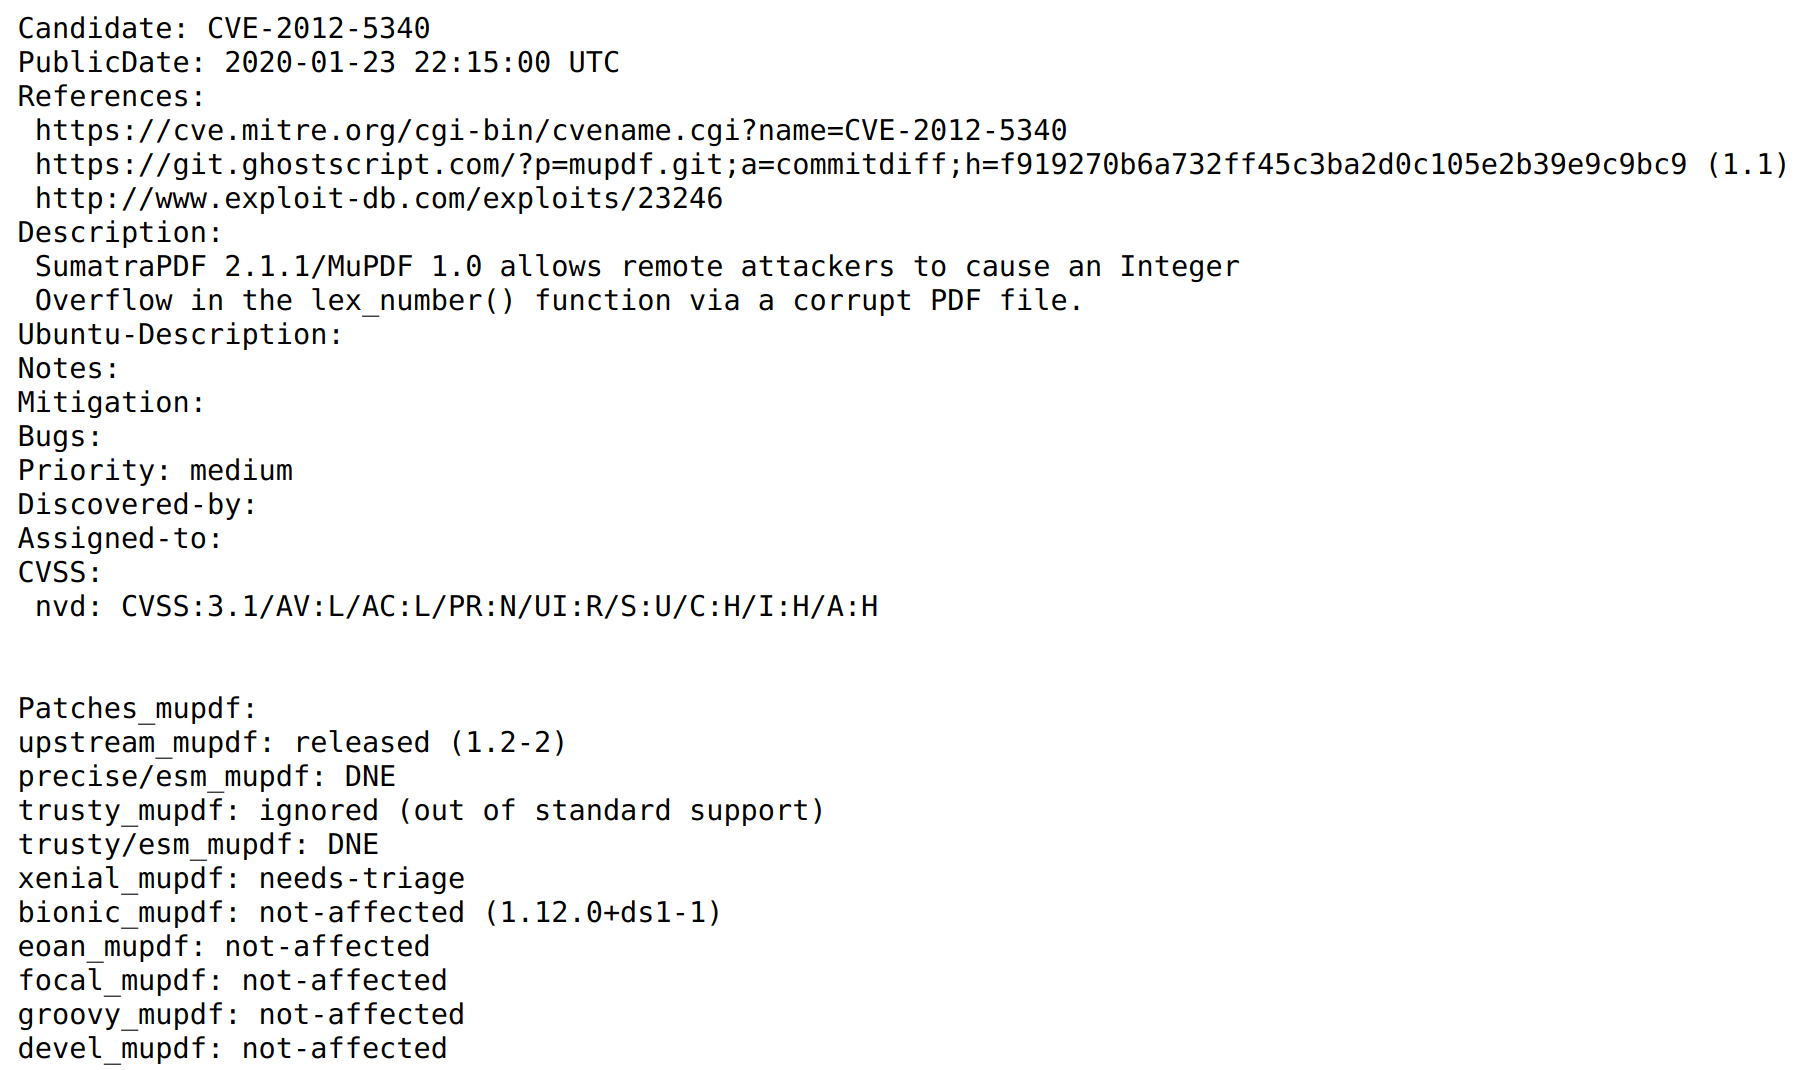
\includegraphics[width=\linewidth]{example.png}}
        \captionof{figure}{Example of a CVE representation in Ubuntu Launchpad Database }
\label{fig:example}
\end{center}

%\subsection{Region 1}
%\begin{enumerate}
%\item\textbf{Linux-libc-dev package-} Out of 4453 vulnerabilities detected by Anchore only (region
%\textbf{1} in Fig~\ref{fig:venn}), 4443 are found in the development
%package of the C library (\texttt{linux-libc-dev} in Ubuntu and Debian).
%Clair detects only Debian vulnerabilities in \texttt{linux-libc-dev},
%whereas Vuls do not detect vulnerabilities in this package at all.
%
%\item\textbf{Vulnerabilities in sub packages-} The
%remaining 10 vulnerabilities in region \textbf{1} are found in sub-packages
%of vulnerable packages: they are correctly reported by Anchore and missed
%by Vuls and Clair.
%
%\subsection{Region 2}
%\begin{enumerate}
%\item\textbf{-} 
%
%
%
\subsection{Discrepancy Reasons}
According to our investigation of these results precisely, below are some of the reasons of
getting different results from these scanners. These reasons include bugs in scanner's logic,
some scanners ignoring vulnerabilities in a particular package, referring to different databases,
how frequently they are updating their database, etc,. We have explained these differences below in detail.
\begin{enumerate}
\item\textbf{Sub-packages vulnerabiities-} Some vulnerabilities in region
	        \textbf{1} are found in sub-packages of vulnerable packages: They are
                 correctly reported by Anchore and missed by Vuls and Clair.

\item\textbf{Linux-libc-dev Package-} Anchore is detecting vulnerabilities in the development
                package of the C library (\texttt{linux-libc-dev} in Ubuntu and Debian). Clair is
		only detecting Debian vulnerabilities in \texttt{linux-libc-dev}, whereas Vuls
		is not detecting vulnerabilities in \texttt{linux-libc-dev} at all. This is the
		reason behind vulnerabilities in region \textbf{1} and region \textbf{2} of the
		Figure~\ref{fig:venn}.

\item \textbf{Vulnerabilities in ESM-} These are the vulnerabilities which are present in Ubuntu 14.04
        ESM release. These vulnerabilities are incorrectly missed by Anchore and Vuls: they have been
         detected in ESM but were already present in LTS. This reason is the main reason for vulnerabilities
	in the region \textbf{3} of the Figure~\ref{fig:venn}.
	 
\item\textbf{Database difference-} Clair is using a Docker image for database. So it is not updated everyday.
                When we scanned images we used the latest available container. For example, CVE-2019-5094 was not
		updated in Clair container that time. This reason adds to region \textbf{3} of the 
		Figure~\ref{fig:venn}.

\item\textbf{Vulnerabilities not in ESM-} Vulnerabilities, which are not present in Ubuntu 14.04 ESM,
	are not detected by Clair but they affect Ubuntu 14.04 LTS, which is present in the image. 
		This is the main reason behind region \textbf{4}
		of the Figure~\ref{fig:venn}.

\item\textbf{Epoch bug-} There is a bug in the Anchore logic due to which some vulnerabilities are
                not detected by Anchore. This bug gets triggered when package’s version have epoch
		(1:3.3.9-1ubuntu2.3) in it. This is one of the major reason behind region \textbf{6}
		of the Figure~\ref{fig:venn}.

\item\textbf{Debian's minor vulnerabilities-} Vulnerabilities marked \texttt{minor}
		 by Debian are ignored by Anchore. However, it is reported by Clair
		  and Vuls. This is also one of the major reason behind region \textbf{6}
		  of the Figure~\ref{fig:venn} in addition to \textit{epoch bug}.

\item\textbf{Out of standard support bug-} There is another bug in Anchore due to
                which it is not able to detect some vulnerabilities. Due to this bug Anchore does not detect
		vulnerabilities which have a status as \texttt{ignored (out of standard support)} in Ubuntu 14.04 LTS.
                This is also one reason behind region \textbf{6} of the Figure~\ref{fig:venn}.

\item\textbf{Ignored (reached end-of-life)-} Some vulnerabilities have status as \texttt{ignored (reached end-of-life)}
                so Anchore checks the last status of these vulnerabilities whether OS package was vulnerable to the cve
                prior to the end-of-life. If it was vulnerable only then Anchore will report it, otherwise not.
                However, Clair may or may not detect it depending on its vulnerability status in ESM release.
		If the vulnerability status is \texttt{DNE( Does Not Exist)} in ESM, Clair does not
		detect it.
		Accordingly, this reason adds vulnerabilities to the region \textbf{6} and \textbf{3} of the Figure~\ref{fig:venn}.

\item\textbf{Rejected CVEs-} There are some CVEs that are rejected because they are duplicate copies of another CVEs.
            Only Vuls is reporting these rejected vulnerabilities. This is one of the reasons behind
		vulnerabilities in the region \textbf{7} of the Figure~\ref{fig:venn}.

\item\textbf{Debian's Temporary vulnerabilities-} Vulnerabilities that are flagged temporary by the
            Debian distribution are reported by Vuls but not by Anchore or
		Clair. This is also one of the reasons that adds to the region \textbf{7} of the Figure~\ref{fig:venn}. 

\item\textbf{Misses by Clair and Anchore-} Clair and Anchore are missing vulnerabilities in Centos images.
	We weren’t able to explain why they were detected by Vuls only. This is the major reason behind
		region \textbf{7} of the Figure~\ref{fig:venn}.
\end{enumerate}
%\subsection{V-C}
%
%V-C represents extra vulnerabilities that are shown by Vuls than Clair.
%So the next question is why they are not shown by Clair then.
%Below are some reasons to answer that question:
%
%
%\begin{enumerate}
%\item\textbf{With Status as “Not-affected”-} It means these vulnerabilities are affecting Ubuntu but they are not
%affecting particular Ubuntu release that is present inside the image. The reason why its not affecting
%that release is also mentioned. For example, one reason can be that code which is creating issue is not
%present in that release etc. In other words, we can say that these vulnerabilities are mistakenly 
%detected by Vuls.
%For example CVE-2015-2305 is not affecting package cups in Trusty.
%
%\item\textbf{Ignored(reached end-of-life)-} These vulnerabilities are ignored in Ubuntu 14.04 LTS as it reached end-of-life
%but does not exist (status as “DNE”) in Ubuntu 14.04 ESM release. As Clair is only referring Ubuntu 14.04 ESM
%release it do not detect these vulnerabilities. For example CVE-2017-9994.
%
%\item\textbf{Not present in Ubuntu 14.04 ESM release-} These vulnerabilities are not present in Ubuntu 14.04 ESM so they
%are not detected by Clair but they affect Ubuntu 14.04 LTS That’s why detected by Vuls. For example, CVE-2017-1375.
%
%\item\textbf{Misses by Clair-} Clair is missing vulnerabilities that it should detect. For example CVE-2016-9082
%is present in package cairo in Ubuntu Xenial release and it is not detected by Clair.
%
%
%\end{enumerate}
%
%\subsection{C-V}
%
%C-V represents extra vulnerabilities that are shown by Clair than Vuls. Following are the reasons to explain that:
%
%\begin{enumerate}
%\item \textbf{Vulnerabilities in Ubuntu 14.04 ESM-} These are the vulnerabilities which are present in Ubuntu 14.04 
%	ESM release. These vulnerabilities are incorrectly missed by Anchore and Vuls: they have been
%         detected in ESM but were already present in LTS.
%%These vulnerabilities are not linked to Ubuntu 14.04 LTS which is
%%present inside the image but Clair is showing because these vulnerabilities are present in Ubuntu 14.04 ESM and
%%Clair is only referring to Ubuntu 14.04 ESM release. For example CVE-2019-1274.
%\item\textbf{Misses by Vuls-} Vuls is missing vulnerabilities that it should detect. For example CVE-2019-5094.
%\end{enumerate}
%
%\subsection{A-C}
%
%A-C represents extra vulnerabilities shown by Anchore than Clair. Below are the reasons:
%\begin{enumerate}
%        \item\textbf{Linux-libc-dev Package-} Clair is not detecting Ubuntu vulnerabilities in the development
%		package of the C library (\texttt{linux-libc-dev}). For example CVE-2019-9506.
%        \item\textbf{Ignored(reached end-of-life)-} These vulnerabilities are ignored in Ubuntu 14.04 LTS as it
%                reached end-of-life but does not exist (DNE) in ESM release. As Clair is only referring
%                Ubuntu 14.04 ESM release it do not detect it. For example CVE-2017-994.
%        \item\textbf{Database difference-} Clair is using a Docker image for database. So it is not updated everyday.
%                When we scanned images we used the latest available container. For example CVE-2019-5094 was not
%                updated in Clair container that time.
%        \item\textbf{Misses by Clair-} Clair is missing vulnerabilities that it should detect. For example
%                CVE-2016-9082 is present in package cairo in Xenial release and it is not detected by Clair.
%\end{enumerate}
%\subsection{C-A}
%C-A represents the vulnerabilities that are not detected by Anchore. Below are the reasons:
%\begin{enumerate}
%
%        \item\textbf{Epoch bug-} There is a bug in the Anchore logic due to which some vulnerabilities are
%                not detected by Anchore. This bug gets triggered when package’s version have epoch
%                (1:3.3.9-1ubuntu2.3)  in it. For example CVE-2018-1125 in procps package.
%        \item\textbf{Ignored (out of standard support) bug-} There is another bug in Anchore due to
%                which it is not able to detect some vulnerabilities. Due to this bug Anchore does not detect
%                vulnerabilities which have a status as “ignored (out of standard support)” in Ubuntu 14.04 LTS.
%                But if this vulnerability is present in Ubuntu 14.04 ESM release it is detected by Clair.
%                For example CVE-2019-13565 in Ubuntu 14.04.
%	\item\textbf{Ignored (reached end-of-life)-} Some vulnerabilities have status as \texttt{ignored (reached end-of-life)}
%                so Anchore checks the last status of these vulnerabilities whether OS package was vulnerable to the cve
%                prior to the end-of-life. If it was vulnerable only then Anchore will report it, otherwise not. But this
%                vulnerability is present in Ubuntu 14.04 ESM release so Clair is reporting that. For example CVE-2019-9924.
%\end{enumerate}
%
%\subsection{A-V}
%
%A-V represents the vulnerabilities that are detected by Anchore but not detected by Vuls. Below are the reasons
%of these differences:
%\begin{enumerate}
%
%        \item\textbf{Linux Package-} Vuls is not detecting all vulnerabilities in the development 
%		package of the C library \textttt{linux-libc-dev in Ubuntu and Debian} . For example CVE-2019-9506.
%        \item\textbf{Misses by Vuls-} Vuls is missing some of the vulnerabilities that it should detect.
%                For example CVE-2019-5094.
%\end{enumerate}
%
%\subsection{V-A}
%V-A represents the vulnerabilities that are detected by Vuls but not detected by Anchore. Below are the reasons:
%\begin{enumerate}
%\item\textbf{Epoch bug-} There is a bug in the Anchore logic due to which some vulnerabilities are not detected
%        by Anchore. This bug gets triggered when package’s version have epoch (1:3.3.9-1ubuntu2.3)  in it.
%                For example CVE-2018-1125 in procps package.
%\item\textbf{Ignored (out of standard support) bug-} There is another bug in Anchore due to which it is not
%        able to detect some vulnerabilities. Due to this bug Anchore does not detect vulnerabilities which
%                have a status as “ignored (out of standard support)” in Ubuntu 14.04 LTS. But these vulnerabilities
%                are detected by Vuls in Ubuntu 14.04 LTS. For example CVE-2019-13565 in Ubuntu 14.04.
%\item\textbf{With status as “Not-affected”-}  It means these vulnerabilities are affecting Ubuntu but they are not
%        affecting particular Ubuntu release that is present inside the image. The reason why its not affecting that
%                release is also mentioned. For example, one reason can be that code which is creating issue is not
%                present in that release etc. For example CVE-2015-2305 is not affecting package cups in Trusty.
%\item\textbf{Rejected CVEs-} There are some CVE that are rejected because they are duplicate copies of another CVEs.
%        So Anchore is not reporting those rejected CVEs but Vuls is reporting those. For example CVE-2017-13753.
%        \end{enumerate}
%
%
\section{Approaches to Reduce Vulnerabilities}

In comparison to tested images, no vulnerabilities were found in latest
updated base
Docker images \texttt{ubuntu:20.04} and \texttt{centos:7}.
So we decided to update these images and see the effect on the
number of vulnerabilities.
Updating an image involves updating all software packages that are
inside that image. However, this option effects the reproducibility
of the image, which means that the image cannot be used to verify research
findings of other scientists. An alternative approach can be to trim unnecessary
packages from images, which in turn reduces the number of vulnerabilities
present in images. Therefore, in this section, we discuss these two
approaches and their effect on the vulnerabilities.

\subsection{Image Update}

A first approach to reduce the number of vulnerabilities in container
images is to update their packages to the latest version available in the OS
distribution. To study the effect of such updates, we developed a script
(available
\href{https://github.com/big-data-lab-team/container-vulnerabilities-paper/blob/master/Scripts/update}{here})
to identify the package manager in the image, and invoke it to update all
OS packages. We updated images on 2019-11-05.

\subsection{Image Minification}

A second approach to reduce the number of vulnerabilities in the images is
to remove unnecessary packages, an operation potentially specific to each
analysis. We used the open-source \reprozip tool~\cite{rampin2016reprozip}
to capture the list of packages used by an analysis. \reprozip first
captures the list of files involved in the analysis, through system call
interception, then retrieves the list of associated software packages, by
querying the package manager. We extend this list with a passlist of
packages required for the system to function, such as \texttt{coreutils}
and \texttt{bash}, and with all the dependencies of the required packages,
retrieved using
\href{http://manpages.ubuntu.com/manpages/xenial/man1/debtree.1.html}{Debtree}.
\href{https://linux.die.net/man/1/repoquery}{Repoquery} could be used in
RPM-based distributions instead. Our minification script, available
\href{https://github.com/big-data-lab-team/container-vulnerabilities-paper/tree/master/Scripts/minification}{here},
installs \reprozip in the image to minify, runs an analysis to collect a
\reprozip trace, and finally deletes all unnecessary packages. We had used
the \href{https://github.com/ReproNim/neurodocker}{Neurodocker} tool
initially, but it did not affect the detected vulnerabilities
as it was removing unused files without using the package manager.

Using this approach, we minified five Debian- or Ubuntu-based BIDS app images,
using basic analysis examples found in the applications documentation.

\subsection{Effect of image update}

Updating container images reduces the number of vulnerabilities by package
by a factor of 3 on average, resulting in only 0.6 extra vulnerabilities by
package (Fig~\ref{fig:update}, r=0.81,
$p\textless10^{-8}$). Twelve container images are missing on this figure:
six of them could not be updated due to various issues with the package
manager, and six of them are Singularity images that we didn't update.
% \change{3 out of these missing 6 images retured an error while updating which
% indicates a problem with the package installer, 2 were unable to update because they
% reached EOL and last one with CentOS 7.1.1503 returned libselinux conflicts with systemd}
In spite of the associated reproducibility challenges, updating
packages therefore appears to be an efficient way to avoid vulnerabilities. It
is not an ultimate solution though, as a substantial number of
vulnerabilities remain.

\begin{center}
\includegraphics[width=\linewidth]{update.pdf}
\captionof{figure}{Number of vulnerabilities by number of
packages, showing a strong linear relationship.}
\label{fig:update}
\end{center}

\subsection{Effect of minification}

Another approach to reduce the number of vulnerabilities involves deleting
unnecessary packages from the container images. It is a tedious operation,
as it requires running an actual data analysis in the container image, to
identify the packages required by the application. In addition, the
resulting container image is only valid for the specific type of analysis
used in the minification process, as other executions might require a
different set of packages.

Using the ReproZip-based approach described previously, we minified 5
different images covering the spectrum of detected vulnerabilities
(Fig~\ref{fig:update_and_minif}). We find that minification reduces the
number of vulnerabilities, albeit less systematically than package update.
For some container images, such as image \textbf{S}, minification removes more
than 70\% of the detected vulnerabilities. For other images, such as
image \textbf{g}, it only reduces the number of vulnerabilities by less than 1\%.
The effect of minification stems from the number of packages
that can be removed, which varies greatly across images. For
instance, images \textbf{g} and \textbf{a} have a large number of packages,
but the last majority of them is required by the analysis, which makes
minification less useful. In other cases, a limited number of unnecessary packages contain
a significant number of vulnerabilities, which makes minification very impactful.
This was the case in images \textbf{d}, \textbf{S} and \textbf{U}, where removing compilers
and kernel headers reduced the number of vulnerabilities by an important fraction.

\subsection{Combined effect of image update and  minification}

Package update and image minification remove different types of
vulnerabilities. The former is efficient against vulnerabilities that have
been fixed by package maintainers, while the latter targets unused
software. In two of the five tested images (images \textbf{S} and \textbf{U}), we find that combining update
and minification further reduces the number of vulnerabilities compared to
using only one of these processes
(Fig~\ref{fig:update_and_minif}).

\begin{center}
\includegraphics[width=\linewidth]{update_and_minif.pdf}
\captionof{figure}{Effect of image minification and
package update on 5 container images, showing that both techniques are
complementary.}
	\label{fig:update_and_minif}
\end{center}

% where do the discrepancies come from?
%We analyzed these results and explained some reasons behind the observed
%discrepancies. Out of 4453 vulnerabilities detected by Anchore only (region
%\textbf{1} in Fig~\ref{fig:venn}), 4443 are found in the development
%package of the C library (\texttt{linux-libc-dev} in Ubuntu and Debian).
%Clair detects only Debian vulnerabilities in \texttt{linux-libc-dev},
%whereas Vuls do not detect vulnerabilities in this package at all. Since Anchore
%ignores Debian
%vulnerabilities flagged as \texttt{minor}, it
%might either detect (region \textbf{2}) or ignore (region \textbf{3})
%the
%Debian vulnerabilities detected by Clair in \texttt{linux-libc-dev}. The
%remaining 10 vulnerabilities in region \textbf{1} are found in sub-packages
%of vulnerable packages: they are correctly reported by Anchore and missed
%by Vuls and Clair.
%
%Many vulnerabilities in region \textbf{3} and \textbf{4} are from images
%based on Ubuntu 14.04. In the Ubuntu CVE tracker database used by Clair and
%Anchore, there are two entries for Ubuntu 14.04: one for LTS (Long-Term
%Support), a Ubuntu release with 5 years of technical support, and another one
%for ESM (Extended Security Maintenance), a release that provides security
%patches beyond the 5 years covered by LTS. Although all the scanned images
%are LTS, Clair refers to the ESM database entry while Anchore and Vuls refer to the
%LTS database entry. The vulnerabilities present in region \textbf{3} due to
%this discrepancy are incorrectly missed by Anchore and Vuls: they have been
%detected in ESM but were already present in LTS. The vulneratibilities in
%region \textbf{4} are incorrectly missed by Clair: they have been fixed in
%ESM but are still present in LTS.
%Some vulnerabilities in region \textbf{6} are due to bugs in Anchore: the
%\textit{epoch bug} ignores vulnerabilities related to package versions that
%contain an epoch (\texttt{:}); the \textit{out of standard bug} ignores
%vulnerabilities that are ignored by the Ubuntu distribution. We reported
%these bugs to the Anchore developers through their Slack channel. Some
%vulnerabilities in region \textbf{6} are also due to the fact that Anchore
%intentionally ignores Debian vulnerabilities flagged as \texttt{minor}.
%
%Finally, 32 vulnerabilities that are flagged temporary by the Debian
%distribution are reported by Vuls but not by Anchore or Clair (region
%\textbf{7}). The remaining 504 vulnerabilities in this region are all found
%in CentOS images. We weren't able to explain why they were detected by Vuls
%only.
